% Options for packages loaded elsewhere
\PassOptionsToPackage{unicode}{hyperref}
\PassOptionsToPackage{hyphens}{url}
\PassOptionsToPackage{dvipsnames,svgnames,x11names}{xcolor}
%
\documentclass[
  number]{elsarticle}

\usepackage{amsmath,amssymb}
\usepackage{iftex}
\ifPDFTeX
  \usepackage[T1]{fontenc}
  \usepackage[utf8]{inputenc}
  \usepackage{textcomp} % provide euro and other symbols
\else % if luatex or xetex
  \usepackage{unicode-math}
  \defaultfontfeatures{Scale=MatchLowercase}
  \defaultfontfeatures[\rmfamily]{Ligatures=TeX,Scale=1}
\fi
\usepackage{lmodern}
\ifPDFTeX\else  
    % xetex/luatex font selection
\fi
% Use upquote if available, for straight quotes in verbatim environments
\IfFileExists{upquote.sty}{\usepackage{upquote}}{}
\IfFileExists{microtype.sty}{% use microtype if available
  \usepackage[]{microtype}
  \UseMicrotypeSet[protrusion]{basicmath} % disable protrusion for tt fonts
}{}
\makeatletter
\@ifundefined{KOMAClassName}{% if non-KOMA class
  \IfFileExists{parskip.sty}{%
    \usepackage{parskip}
  }{% else
    \setlength{\parindent}{0pt}
    \setlength{\parskip}{6pt plus 2pt minus 1pt}}
}{% if KOMA class
  \KOMAoptions{parskip=half}}
\makeatother
\usepackage{xcolor}
\setlength{\emergencystretch}{3em} % prevent overfull lines
\setcounter{secnumdepth}{5}
% Make \paragraph and \subparagraph free-standing
\makeatletter
\ifx\paragraph\undefined\else
  \let\oldparagraph\paragraph
  \renewcommand{\paragraph}{
    \@ifstar
      \xxxParagraphStar
      \xxxParagraphNoStar
  }
  \newcommand{\xxxParagraphStar}[1]{\oldparagraph*{#1}\mbox{}}
  \newcommand{\xxxParagraphNoStar}[1]{\oldparagraph{#1}\mbox{}}
\fi
\ifx\subparagraph\undefined\else
  \let\oldsubparagraph\subparagraph
  \renewcommand{\subparagraph}{
    \@ifstar
      \xxxSubParagraphStar
      \xxxSubParagraphNoStar
  }
  \newcommand{\xxxSubParagraphStar}[1]{\oldsubparagraph*{#1}\mbox{}}
  \newcommand{\xxxSubParagraphNoStar}[1]{\oldsubparagraph{#1}\mbox{}}
\fi
\makeatother


\providecommand{\tightlist}{%
  \setlength{\itemsep}{0pt}\setlength{\parskip}{0pt}}\usepackage{longtable,booktabs,array}
\usepackage{calc} % for calculating minipage widths
% Correct order of tables after \paragraph or \subparagraph
\usepackage{etoolbox}
\makeatletter
\patchcmd\longtable{\par}{\if@noskipsec\mbox{}\fi\par}{}{}
\makeatother
% Allow footnotes in longtable head/foot
\IfFileExists{footnotehyper.sty}{\usepackage{footnotehyper}}{\usepackage{footnote}}
\makesavenoteenv{longtable}
\usepackage{graphicx}
\makeatletter
\def\maxwidth{\ifdim\Gin@nat@width>\linewidth\linewidth\else\Gin@nat@width\fi}
\def\maxheight{\ifdim\Gin@nat@height>\textheight\textheight\else\Gin@nat@height\fi}
\makeatother
% Scale images if necessary, so that they will not overflow the page
% margins by default, and it is still possible to overwrite the defaults
% using explicit options in \includegraphics[width, height, ...]{}
\setkeys{Gin}{width=\maxwidth,height=\maxheight,keepaspectratio}
% Set default figure placement to htbp
\makeatletter
\def\fps@figure{htbp}
\makeatother

\makeatletter
\@ifpackageloaded{caption}{}{\usepackage{caption}}
\AtBeginDocument{%
\ifdefined\contentsname
  \renewcommand*\contentsname{Table of contents}
\else
  \newcommand\contentsname{Table of contents}
\fi
\ifdefined\listfigurename
  \renewcommand*\listfigurename{List of Figures}
\else
  \newcommand\listfigurename{List of Figures}
\fi
\ifdefined\listtablename
  \renewcommand*\listtablename{List of Tables}
\else
  \newcommand\listtablename{List of Tables}
\fi
\ifdefined\figurename
  \renewcommand*\figurename{Figure}
\else
  \newcommand\figurename{Figure}
\fi
\ifdefined\tablename
  \renewcommand*\tablename{Table}
\else
  \newcommand\tablename{Table}
\fi
}
\@ifpackageloaded{float}{}{\usepackage{float}}
\floatstyle{ruled}
\@ifundefined{c@chapter}{\newfloat{codelisting}{h}{lop}}{\newfloat{codelisting}{h}{lop}[chapter]}
\floatname{codelisting}{Listing}
\newcommand*\listoflistings{\listof{codelisting}{List of Listings}}
\makeatother
\makeatletter
\makeatother
\makeatletter
\@ifpackageloaded{caption}{}{\usepackage{caption}}
\@ifpackageloaded{subcaption}{}{\usepackage{subcaption}}
\makeatother

\ifLuaTeX
  \usepackage{selnolig}  % disable illegal ligatures
\fi
\usepackage[]{natbib}
\bibliographystyle{elsarticle-num}
\usepackage{bookmark}

\IfFileExists{xurl.sty}{\usepackage{xurl}}{} % add URL line breaks if available
\urlstyle{same} % disable monospaced font for URLs
\hypersetup{
  pdftitle={Draft -- Effect of Atmospheric Heatwaves on Reflectance and Pigment Composition of Intertidal Nanozostera noltei -- Draft},
  pdfauthor={Simon Oiry; Bede Ffinian Rowe Davies; Philippe Rosa; Augustin Debly; Anne-Laure Barillé; Nicolas Harrin; Pierre Gernez; Laurent Barillé},
  pdfkeywords={Remote Sensing, Pigment Composition, Seagrass, Coastal
Ecosystems, Heatwaves},
  colorlinks=true,
  linkcolor={blue},
  filecolor={Maroon},
  citecolor={Blue},
  urlcolor={Blue},
  pdfcreator={LaTeX via pandoc}}


\setlength{\parindent}{6pt}
\begin{document}

\begin{frontmatter}
\title{Draft -- Effect of Atmospheric Heatwaves on Reflectance and
Pigment Composition of Intertidal \emph{Nanozostera noltei} -- Draft}
\author[1]{Simon Oiry%
\corref{cor1}%
}
 \ead{oirysimon@gmail.com} 
\author[1]{Bede Ffinian Rowe Davies%
%
}

\author[1]{Philippe Rosa%
%
}

\author[1]{Augustin Debly%
%
}

\author[2]{Anne-Laure Barillé%
%
}

\author[2]{Nicolas Harrin%
%
}

\author[1]{Pierre Gernez%
%
}

\author[1]{Laurent Barillé%
%
}


\affiliation[1]{organization={Institut des Substances et Organismes de
la Mer, ISOMer, Nantes Université, UR 2160, F-44000 Nantes,
France},,postcodesep={}}
\affiliation[2]{organization={Bio-littoral, Immeuble Le Nevada, 2 Rue du
Château de l'Eraudière, 44300 Nantes, France},,postcodesep={}}

\cortext[cor1]{Corresponding author}








        
\begin{abstract}
To be written
\end{abstract}





\begin{keyword}
    Remote Sensing \sep Pigment Composition \sep Seagrass \sep Coastal
Ecosystems \sep 
    Heatwaves
\end{keyword}
\end{frontmatter}
    

\section{Introduction}\label{introduction}

Intertidal seagrasses play a crucial role in the ecosystem by providing
habitats and feeding grounds for various marine species, supporting rich
marine biodiversity, and contributing significantly to primary
production and carbon sequestration
\citep{unsworth2022planetary, sousa2019blue}. These seagrasses are
essential in maintaining the health of coastal ecosystems by stabilizing
sediments, filtering water, and serving as indicators of environmental
changes due to their sensitivity to water quality variations
\citep{zoffoli2021decadal}. The interactions between seagrass meadows
and their associated herbivores further enhance the delivery of
ecosystem services, including coastal protection and fisheries support
\citep{jankowska2019stabilizing, zoffoli2023remote, gardner2018global}.
Understanding and preserving these ecosystems are vital for maintaining
the biodiversity and productivity of coastal regions
\citep{scott2018role, ramesh2020seagrass}.

Despite their crucial role in marine ecosystems, intertidal seagrasses
face numerous threats that compromise their health and functionality.
Coastal development and human activities are primary threats. These
activities not only reduce the available habitat for seagrasses but also
increase water turbidity, which limits light penetration and hampers
photosynthesis \citep{waycott2009accelerating}. Seagrasses are also
threatened by nutrient enrichment from agricultural and urban runoff,
which can lead to eutrophication. This condition promotes the overgrowth
of algal blooms that compete with seagrasses for light and nutrients,
further stressing these important plants \citep{thomsen2023meadow} (Oiry
et al.~2024). Pollution from industrial and agricultural fields sources
introduces harmful chemicals and heavy metals into coastal waters,
posing toxic risks to seagrass health. These pollutants can affect the
physiological processes of seagrasses, reducing their growth and
survival rates \citep{sevgi2022bitkilerde} Additionally, invasive
species can out compete native seagrasses for resources, altering
community structure and function \citep{simpson2016distribution}.

Heatwaves, exacerbated by climate change, pose a growing threat to
seagrasses. Marine Heatwaves (MHW), defined by
\citep{hobday2016hierarchical} as prolonged discrete anomalously warm
water events, and Atmospheric Heatwaves (AHW), defined by
\citep{perkins2013measurement} as periods of at least three consecutive
days with temperatures exceeding the 90th percentile, cause severe
physiological stress on seagrasses
\citep{sawall2021chronically, deguette2022physiological}. At the
interface between the land and oceans, intertidal seagrasses are exposed
to both MHW and AHW. Heatwaves have profound impacts on seagrasses, with
their effects varying based on species and geographic location. For
instance, the seagrass \emph{Zostera marina} exhibits high
susceptibility to elevated sea surface temperatures during winter and
spring, leading to advanced flowering, high mortality rates, and reduced
biomass \citep{sawall2021chronically}. Similarly, \emph{Cymodocea
nodosa} shows increased photosynthetic activity during heatwaves but
suffers negative effects on photosynthetic performance and leaf biomass
during recovery \citep{deguette2022physiological}. Additionally,
different populations of \emph{Zostera marina} along the European
thermal gradient exhibit varied photophysiological responses during the
recovery phase of heatwaves, indicating differential adaptation
capabilities among populations \citep{winters2011effects}. These events
intensify other stressors, such as overgrazing and seed burial,
compromising sexual recruitment \citep{guerrero2020heat}.

Bleaching and darkening events of seagrass beds have been observed
following episodes of intense heat along the Brittany coast of France
(Pers. obs.) then affecting leaf color, which are expected to alter leaf
reflectance. Remote sensing is increasingly being utilized to monitor
marine ecosystems, including seagrass meadows. By using spectral
indices, such as the Normalized Difference Vegetation Index (NDVI) and
the Soil-Adjusted Vegetation Index (SAVI), or by analyzing specific
spectral patterns, remote sensing can effectively quantify vegetation
health over time
\citep{huete2012vegetation, kloos2021agricultural, carlan2020identifying, akbar2020mangrove}.
Through the Water Framework Directive and the Marine Strategy Framework
Directive, Europe is promoting remote sensing techniques for habitat
mapping, as these methods enable the monitoring of extensive areas over
time \citep{papathanasopoulou2019satellite}. This study will
experimentally test the hypothesis that warm events modify the pigment
composition and reflectance of seagrass, linking these changes with
satellite remote sensing.

\section{Material \& Methods}\label{material-methods}

\subsection{\texorpdfstring{\emph{in situ} observation of seagrass
leaves
darkening.}{in situ observation of seagrass leaves darkening.}}\label{in-situ-observation-of-seagrass-leaves-darkening.}

\subsubsection{Field campaign}\label{field-campaign}

\phantomsection\label{cell-fig-quiberonMap}
\begin{figure}[H]

\centering{

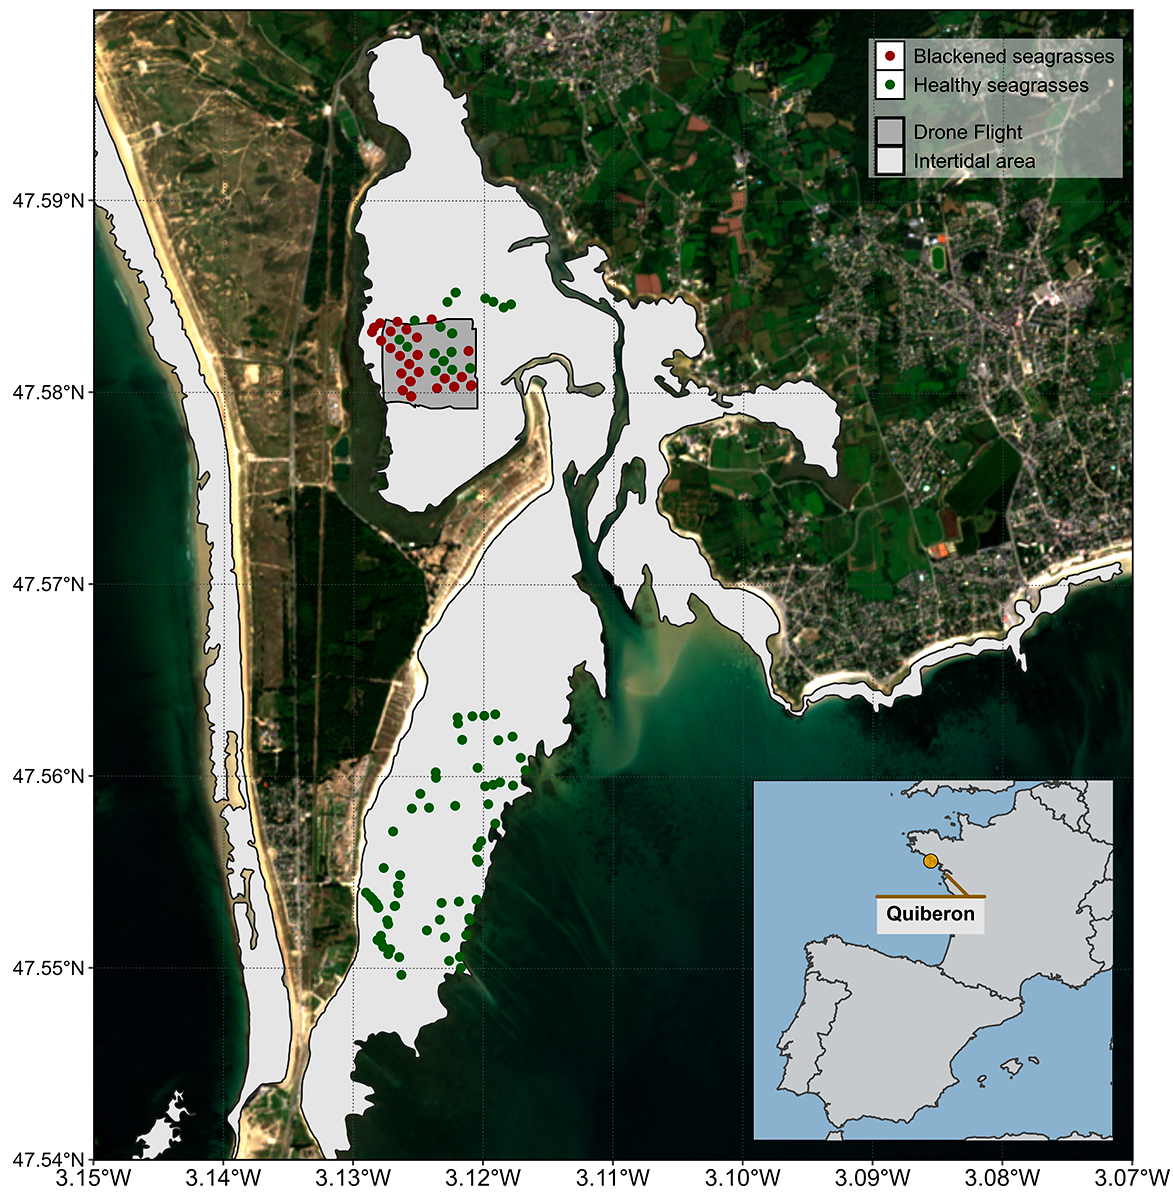
\includegraphics[width=1\textwidth,height=\textheight]{Figs/Quiberon_map.png}

}

\caption{\label{fig-quiberonMap}Location of the fieldtrip campaign that
occured in the 10th of September 2021. The light grey polygons indicates
the intertidal zone (Zone between High tide and low tide, that is
totally emerged at low tide) and the dark grey polygon indicate the
extent of the drone flight. Green dots indicate location of quadrat
picture over healthy seagrasses while red dots indicate location of
quadrat took over darkened seagrasses.}

\end{figure}%

A fieldtrip, aiming to map a seagrass meadow near Quiberon (France :
46°57'32.0''N, 2°10'37.0''W), occurred in the 10th of September 2021
Figure~\ref{fig-quiberonMap}. During this fieldtrip, darkening of
seagrasses have been observed, resulting in the darkening of seagrass
leaves over large area of the meadow Figure~\ref{fig-QuiberonImg}.
During this field trip, drone flights were conducted over two areas of
the seagrass meadow using a DJI Matrice 200 equipped with a Sequoia
Multispectral camera. The Sequoia captures four spectral bands: Green
(550 ± 40 nm), Red (660 ± 40 nm), RedEdge (735 ± 10 nm), and Near
Infrared (790 ± 40 nm). A total of 285 Ground Control Points (GCPs) were
collected in the form of georeferenced quadrat images across the meadow
. These images allow for visual assessment of vegetation type, density,
and health status. The images were then divided into two categories:
Healthy seagrasses and darkened seagrasses, based on a visual estimation
of the leaf condition Figure~\ref{fig-quiberonMap}.

\phantomsection\label{cell-fig-QuiberonImg}
\begin{figure}[H]

\centering{

\includegraphics[width=1\textwidth,height=\textheight]{Figs/img_Quiberon.png}

}

\caption{\label{fig-QuiberonImg}Illustrations of the two health
conditions of seagrasses observed in the field. A: Global view of a
healthy green meadow; B: Quadrat images of healthy seagrasses; C:
Quadrat images of darkened seagrasses; D: Global view of an unhealthy
darkened meadow. All images were taken on September 10th, 2021, in
Quiberon.}

\end{figure}%

\subsubsection{Temparature Data and identification of
heatwaves}\label{temparature-data-and-identification-of-heatwaves}

\paragraph{Air temperature}\label{air-temperature}

Since January 1, 2024, Meteo France weather data has been freely and
openly accessible. Hourly air temperature data (°C) for the French
Atlantic and Channel coasts was retrieved using a
\href{https://github.com/SigOiry/HeatWave_Seagrasses/blob/main/Scripts/MeteoFrance_Extraction.qmd}{custom
script} as no API was available at the time of this study. Weather
stations located within 10 kilometers of the coastline were considered,
but only those with at least 30 years of data were included to ensure
reliable climatological reconstruction. Of the 156 weather stations
within 10 kilometers of the coast, only 36 had sufficient data for
climatology reconstruction. The hourly data was then aggregated into
daily mean temperatures for each station.

Heatwave detection was performed using the HeatwaveR package in R
\citep{heatwaveR}. This package utilizes the methodology proposed by
\citep{hobday2016hierarchical} to detect heatwave events. The
climatology for the year was computed using the temperature time series.
An event was considered a heatwave each time the temperature exceeded
the 90th percentile of the climatology for three consecutive days. The
severity of each event has been assessed using the methodology proposed
by \citep{hobday2018categorizing}.

\paragraph{Water temperature}\label{water-temperature}

Sea Surface Temperature (SST) data were downloaded from the Copernicus
CMEMS platform \citep{CMEMS_1} for the French coast, covering the period
from 1982 to 2022. Only pixels within an area of 2700 km² around
Quiberon, Brittany, France (47°29′03″N, 3°07′09″W) were extracted and
analyzed. This area was large enough to minimize missing values caused
by cloud cover, yet small enough to avoid being influenced by the
stability of offshore SST. After the masking step, a daily average of
the remaining pixels was calculated, resulting in a daily mean SST value
for the entire time series. Using this daily average since 1982, the SST
climatology was computed with the HeatwaveR package in R
\citep{heatwaveR}. The same methodology used to detect air temperature
events was applied to identify SST events.

\subsection{Laboratory experiment}\label{laboratory-experiment}

\subsubsection{Sampling and acclimation of
seagrasses}\label{sampling-and-acclimation-of-seagrasses}

Seagrass was sampled from a \emph{Nanozostera noltei} (dwarf eelgrass,
syn. \emph{Zostera noltei}) meadow on Noirmoutier Island, France
(46°57'32.0''N, 2°10'37.0''W) at low tide in June 2024. A home-made inox
sampling box was used to sample seagrass from an area of 30 cm by 15 cm
and 5 cm deep, maintaining the sediment structure and avoiding damage to
the rhizomes and the leafs of the seagrass (Figure~\ref{fig-design} A).
This sampling box allowed to limitate sampling variability between
replicates. The seagrass, along with sediment, meiofauna, and
macrofauna, was placed in plastic trays. To avoid hydric stress during
transportation, seawater was added to each tray. Simultaneously,
seawater was sampled from a nearby site and transported to the lab,
where it was filtered using a 0.22 µm nitrocellulose filter to remove
all suspended particulate matter. This seawater was used in the
acclimation tank and the intertidal chambers. The seagrasses were
acclimated at high tide for one weeks with a water temperature of 17°C,
matching the temperature at the time of sampling, and with light of 150
µmol.s-1.m-2 of PAR photons \citep{akbar2020mangrove}. A wave generator
was used in the tank to circulate and reoxygenate the water.

\subsubsection{Experimental design}\label{experimental-design}

\phantomsection\label{cell-fig-design}
\begin{figure}[H]

\centering{

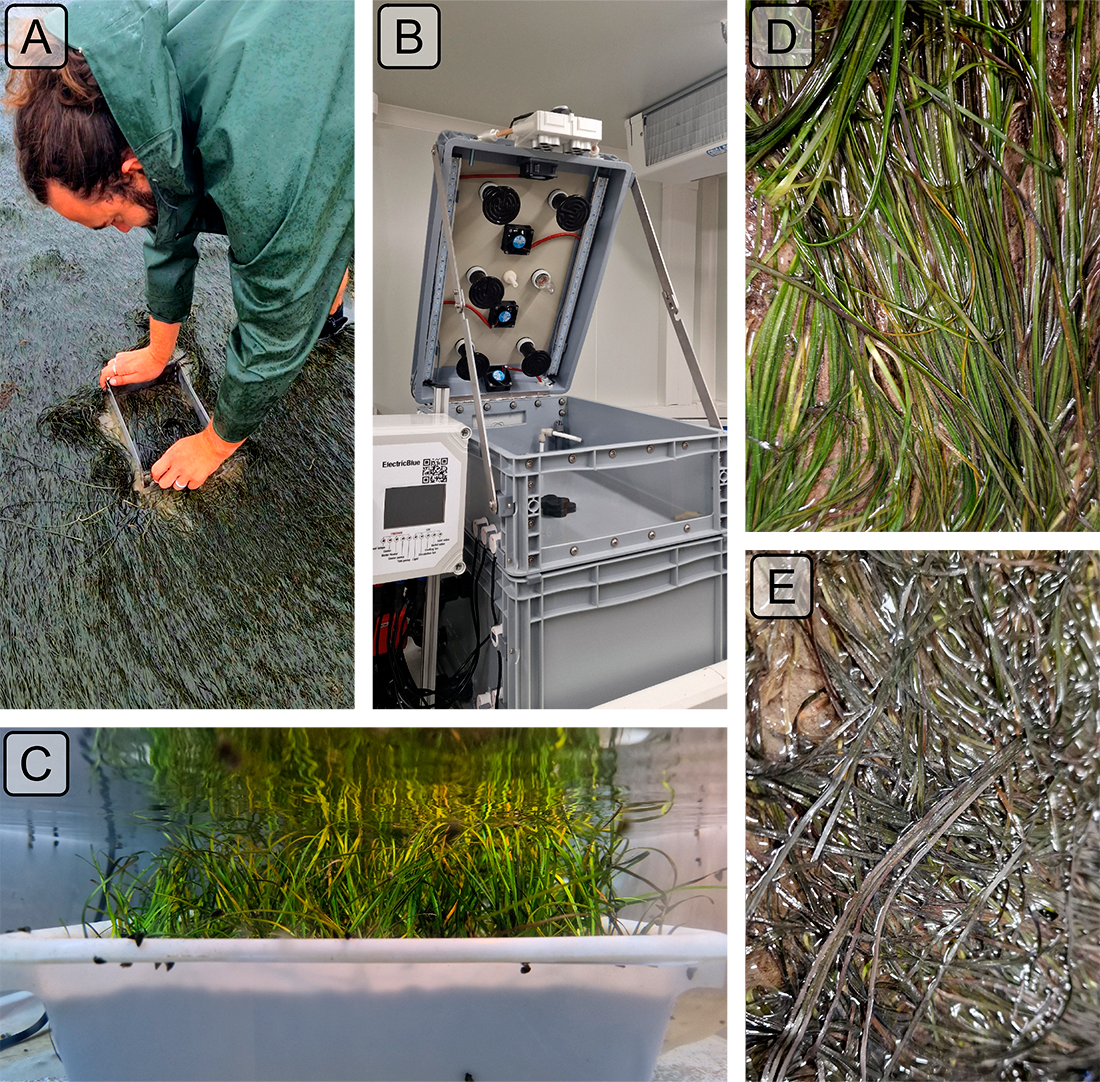
\includegraphics[width=1\textwidth,height=\textheight]{Figs/Experimental_design.png}

}

\caption{\label{fig-design}Illustrations of the various steps of the
experiment. A: Field sampling of seagrass using a homemade sampling box;
B: Intertidal chambers used during the experiment; C: Seagrass sample
inside a chamber during the experiment at high tide; D: Photo of the
treatment sample at the start of the experiment; E: Photo of the
treatment sample at the end of the experiment.}

\end{figure}%

Two intertidal chambers from
\href{https://electricblue.eu/intertidal-chamber}{ElectricBlue} were
used to simulate tidal cycles and control water temperature during high
tide and air temperature during low tide (Figure~\ref{fig-design} B,C).
One chamber served as the control, while the other was used for the
experimental treatment. The control chamber was maintained at
temperatures representative of the typical seasonal conditions: water
temperatures between 18°C and 19°C and air temperatures between 18°C and
23°C, following circadian temperature variability
(Figure~\ref{fig-Profile} left). For the experimental treatment, the air
temperature was set to mimic an atmospheric heatwave that occurred over
the seagrass meadow of Porh Saint-Guénël, Plouharnel, France
(47°35'40.0''N, 3°07'30.0''W) from August 26, 2021, to September 6,
2021. On the first day of the experiment, air temperatures in the
experimental chamber were set to range from 23°C at night to 35°C during
the day, with a daily increase of 1°C. The water temperature in the
experimental chamber was similarly adjusted to reflect the heatwave
conditions, starting from the normal seasonal range (18°C) and gradually
increasing to simulate the rising temperatures experienced during the
heatwave (+0.5°C daily). This setup aimed to replicate the thermal
stress experienced by the seagrass meadow during the actual heatwave
event (Figure~\ref{fig-Profile} right).

\phantomsection\label{cell-fig-Profile}
\begin{figure}[H]

\centering{

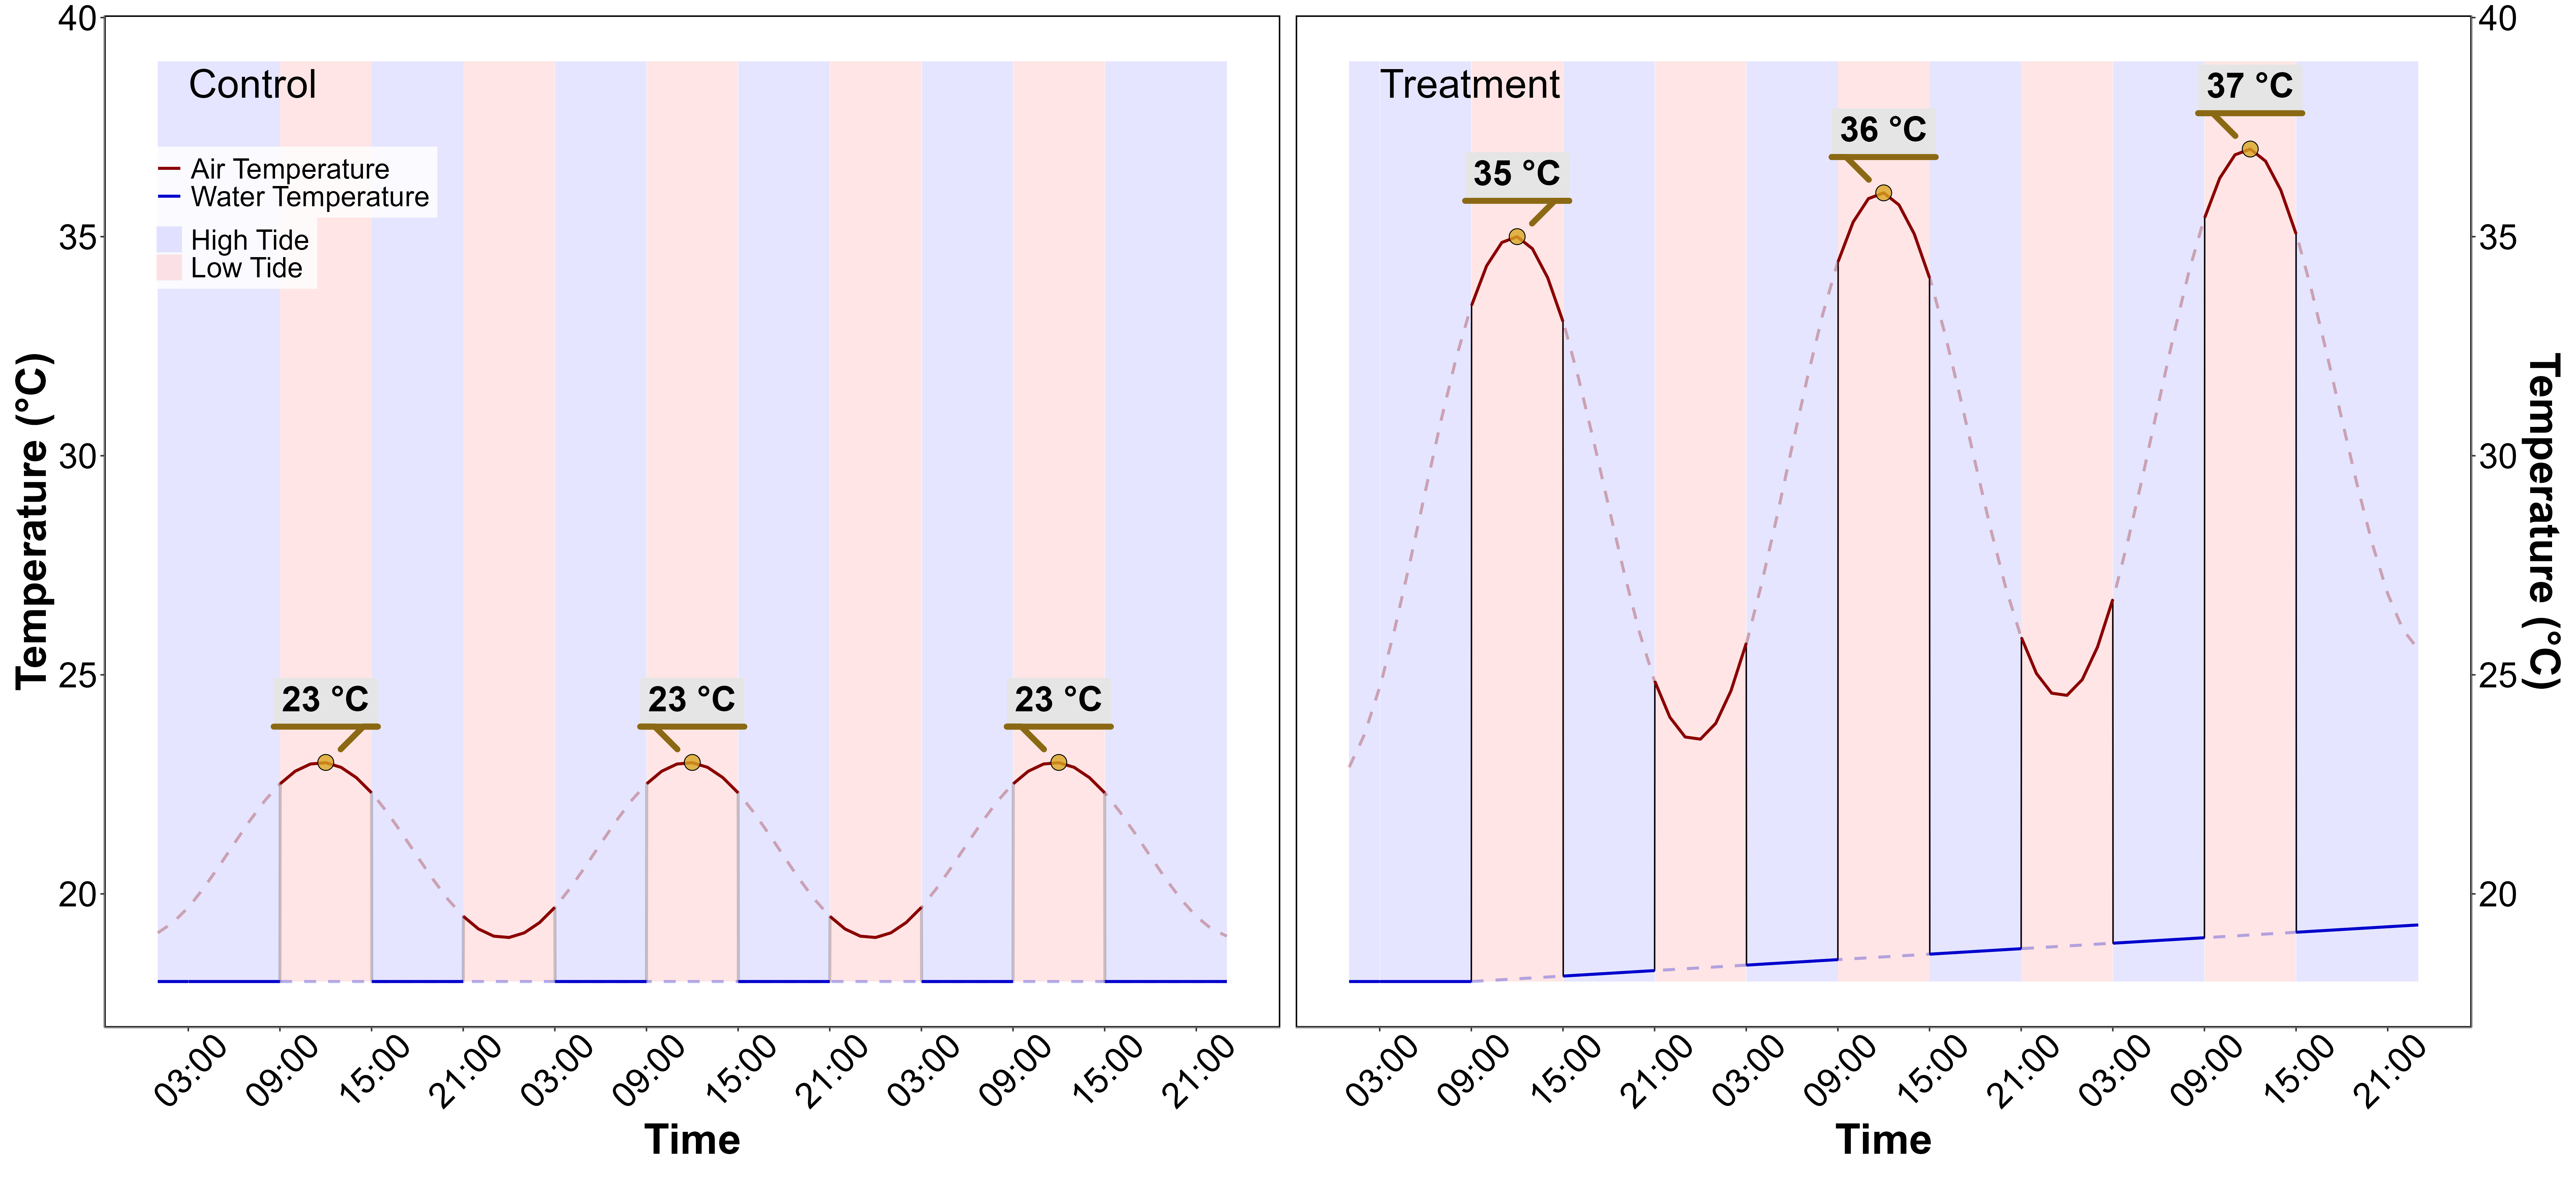
\includegraphics[width=1\textwidth,height=\textheight]{Figs/Chamber_Profils.png}

}

\caption{\label{fig-Profile}Temperature profiles of both the control
(left) and the treatment (right) followed during the heatwave
experiment. The red line indicates air temperature, whereas the blue
line indicates water temperature. Due to the tidal cycle followed during
the experiment, the seagrasses only experience temperatures representade
by solid lines.}

\end{figure}%

\subsubsection{Bio-optical measurmenents over seagrass
leaves}\label{bio-optical-measurmenents-over-seagrass-leaves}

\paragraph{Hyperspectral measurements}\label{hyperspectral-measurements}

Throughout the experiment, hyperspectral signatures of both the control
and treatment seagrasses were taken using an ASD HandHeld 2 equipped
with a fiber optic, allowing measurements to be taken directly inside
the chamber without opening it. Automatic spectra acquisition has been
done using the
\href{https://www.malvernpanalytical.com/en/learn/knowledge-center/user-manuals/rs3-software-user-manual}{RS3
softaware} developed by the intrument manufacturer. An average of five
reflectance spectrum (\(R(\lambda)\)), each with an integration time of
544 ms, was taken every minute. Every 10 minutes, the fiber optic was
switched from one benthic chamber to the other, in order to measure
reflectance in both treatment and control. Because light conditions were
controlled inside of the chambers, reflectance calibration of the
instrument was performed only each morning at the very first moment of
low tide using a Spectralon white reference with 99\% Lambertian
reflectivity.

The second derivative of \(R\) was calculated to retrieve absorption
features and compare their variability over time. Two radiometric
indices were also monitored throughout the experiment :

\begin{itemize}
\tightlist
\item
  The Normalized Difference Vegetation Index (NDVI,
  \citep{rouse1974monitoring}), as a proxy of the concentration of
  chlorophyll-a (Equation~\ref{eq-ndvi})
\end{itemize}

\begin{equation}\phantomsection\label{eq-ndvi}{
NDVI = \frac{R(840)-R(668)}{R(840)+R(668)}
}\end{equation}

where \(R(840)\) and \(R(668)\) are the reflectance at 840 nm and 668 nm
respectively.

\begin{itemize}
\tightlist
\item
  The Green Leaf Index (GLI, \citep{louhaichi2001spatially}), as a
  measurement of the greenness of seagrass leafs (Equation~\ref{eq-gli})
\end{itemize}

\begin{equation}\phantomsection\label{eq-gli}{
GLI = \frac{[R(550)-R(668)]+[R(550)-R(450)]}{(2 \times R(550) )+ R(668) + R(450) }
}\end{equation}

where \(R(550)\) and \(R(450)\) are the reflectance in green at 550 nm
and in the blue at 450 nm, respectively.

\begin{itemize}
\tightlist
\item
  The Mid-Infrared Water Absorption Index (MIWAI), proposed here and
  designed to measure water absorption at 970 nm (\textbf{REF}),
  estimates the difference between the reflectance at 970 nm and a
  linear interpolation of the reflectance values at 950 and 990 nm. This
  interpolation represents the expected reflectance value in the absence
  of water.
\end{itemize}

\begin{equation}\phantomsection\label{eq-MIWAI}{
MIWAI = 0.5 \times [R(990)+R(950)]-R(970)
}\end{equation}

where \(R(990)\), \(R(970)\) and \(R(950)\) are the reflectance in the
infrared at 990, 970 and 950 nm, respectively.

\begin{quote}
\mbox{}%
\paragraph{Multispectral imagery
measurement}\label{multispectral-imagery-measurement}

Parallel to hyperspectral measurements, multispectral images were taken
at the beginning and end of each diurnal low tide (09:00 am and 03:00
pm). A Micasense RedEdge-MX Dual multispectral camera, originally
designed to be mounted on a drone, was modified for use without a drone.
A 3D-printed mount was designed to attach the camera to the intertidal
chamber and ensure that each picture was captured under the same
conditions. At each time step (09:00 am and 03:00 pm), a first picture
of the Spectralon was taken to allow for image correction in
reflectance, followed by a second picture of the target.
\href{https://sigoiry.github.io/DISCOV-MicaSense/}{DISCOV}, a Neural
Network classification model previously developed to map intertidal
vegetation using drone imagery, has been applied to each image taken
inside the intertidal chambers. To understand the behavior of the model
on seagrasses affected by heatwaves, classification images from before
and after the heatwave have been compared.
\end{quote}

\paragraph{Pigment concentration
measurements}\label{pigment-concentration-measurements}

At the beginning and the end of each diurnal low tide (09:00 am and
03:00 pm) leaves samples have been took in both the test and the
control. leaves sampled have been stored under -80°C waiting for
analysis. Pigment composition and biomass were analyzed using
high-performance liquid chromatography (HPLC). The HPLC system (Alliance
HPLC 248 System, Waters) was equipped with a reverse-phase C-18
separating column (SunFire C-18 Column, 100Å, 3.5 µm, 2.1 mm x 50 mm,
Waters), preceded by a precolumn (VanGuard 3.9 mm x 5 mm, Waters). The
system also included a photodiode array detector (2998 PDA) and a
fluorimeter (Ex: 425 nm, Em: 655 nm; RF-20A, SHIMADZU).

\textbf{Au secours Philippe !!!}

\section{Results}\label{results}


\renewcommand\refname{Bibliography}
  \bibliography{library.bib}



\end{document}
